% Chapter Template

\chapter{Ensayos y Resultados} % Main chapter title
\label{Chapter4}

En este capítulo se presentan las pruebas realizadas para validar el correcto funcionamiento del sistema implementado. Se incluyen pruebas funcionales de cada bloque en particular y también de todo el sistema integrado.

\section{Pruebas funcionales}

A medida que se desarrollaron los diferentes módulos del firmware del sistema, se llevaron a cabo las correspondientes pruebas en cada uno de ellos, para validar que funcionaban de la manera esperada antes de ser integrados con otras partes del sistema. Todas las pruebas fueron realizadas manualmente.

Los bloques a probar se pueden dividir en tres: la comunicación por WiFi, la comunicación utilizando BLE y la comunicación con el electrodoméstico.

\subsection{Comunicación WiFi}

La comunicación por WiFi es la parte del sistema más compleja y la que por lo tanto requiere pruebas más exhaustivas de sus diferentes funcionalidades.

Independientemente de la aplicación que se le vaya a dar, el primer paso es lograr conectarse exitosamente a una red WiFi. Esta fue la primera prueba realizada, configurando a mano las credenciales de la red inalámbrica y verificando por consola que se conecte correctamente, como se puede ver en la figura \ref{fig:output_wifi_connection}. En ella, se ve que se inició la conexión y luego se registró el evento en el que el microcontrolador obtuvo una dirección IP y por lo tanto se conectó con éxito.

\begin{figure}[h]
\centering
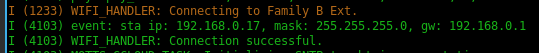
\includegraphics[width=\textwidth]{./Figures/output_wifi_connection.png}
\caption{Salida por consola del microcontrolador al conectarse a una red WiFi.}
\label{fig:output_wifi_connection}
\end{figure}

Una vez llegado a este punto, es posible continuar con las pruebas asociadas a la comunicación con el usuario del electrodoméstico, mediante una interfaz de usuario, y con el fabricante, enviando información hacia Google Cloud.

\subsubsection{Comunicación con el usuario}

Si bien en los alcances del trabajo se especificó que no se incluía el desarrollo de una interfaz web desde la cual el usuario pudiese interactuar con el electrodoméstico, de todos modos se requiere contar con algún mecanismo para enviar comandos desde Internet para verificar el correcto funcionamiento. Por ello es que se recurrió a diferentes plataformas web IoT configurables ya existentes.

Para las pruebas de envío y recepción mediante los protocolos HTTP y HTTPS, se utilizó ThingSpeak \citep{thingspeak}. Esta plataforma permite recibir información desde el microcontrolador, almacenarla y graficarla. Además permite enviar comandos desde la página hacia el microcontrolador. Si bien ThingSpeak ofrece una librería para interactuar con la plataforma, en este caso se utilizaron directamente las direcciones indicadas en su documentación para enviar HTTP \emph{requests} desde las tareas de transmisión y recepción WiFi que se ejecutan en el microcontrolador. De esta forma por un lado se enviaron comandos desde ThingSpeak y se observó por consola que el microcontrolador los recibía correctamente. Por otro lado se enviaron datos periódicamente hacia ThingSpeak y se los graficó, verificando que tienen los valores esperados.

Para demostrar la versatilidad del módulo desarrollado, se decidió utilizar una plataforma IoT diferente para probar la comunicación utilizando MQTT. Por eso se utilizó Adafruit IO \citep{adafruit}, plataforma que permite crear tableros o \emph{dashboards} personalizados para comunicarse con sistemas embebidos. La figura \ref{fig:adafruit_dashboard} muestra la interfaz desarrollada, en la que se puede ver que se tienen diferentes botones para enviar comandos determinados, un historial de comandos enviados, un cuadro mostrando el estado del electrodoméstico (\emph{slave}) y un cuadro con el último comando enviado.

\begin{figure}[h]
\centering
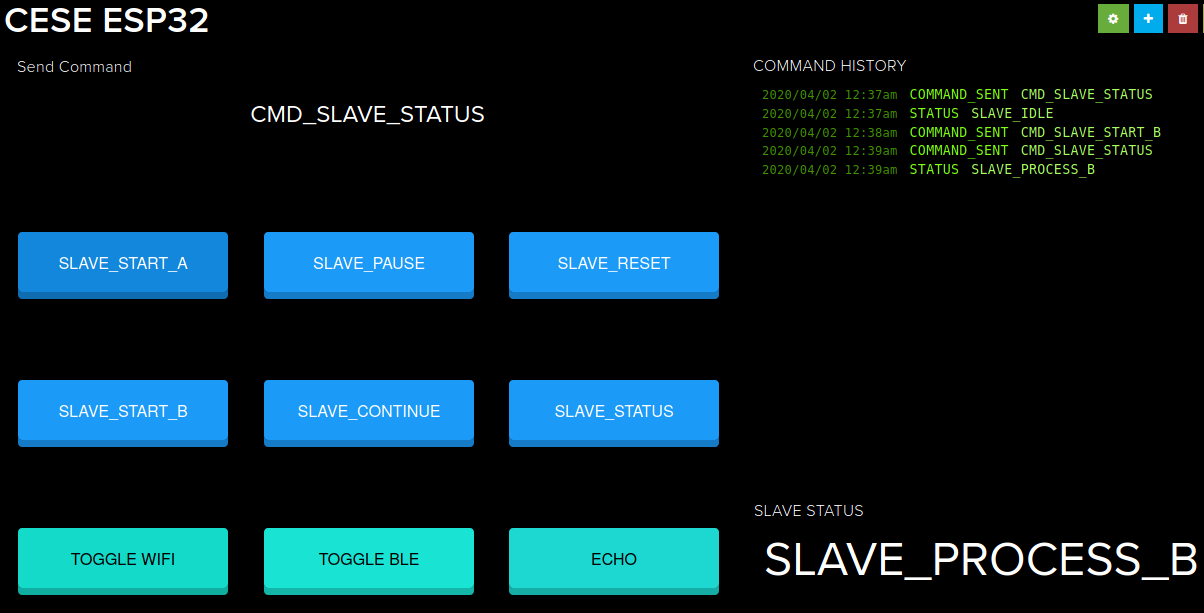
\includegraphics[width=\textwidth]{./Figures/adafruit_dashboard.png}
\caption{Interfaz de usuario creada en Adafruit IO.}
\label{fig:adafruit_dashboard}
\end{figure}

En el historial de comandos se puede observar que se envió un comando para conocer el estado del electrodoméstico (CMD\_SLAVE\_STATUS) y se recibió de vuelta el estado actual (SLAVE\_IDLE, es decir inactivo sin ejecutar ninguna acción). Luego se envió un comando para iniciar un proceso en el electrodoméstico (CMD\_SLAVE\_PROCESS\_B), y al preguntar nuevamente por el estado, se obtuvo que se encontraba ejecutando la acción iniciada con el comando anterior.

Desde el punto de vista del firmware, en la figura \ref{fig:output_mqtt_connection} se observa cómo van ocurriendo los diferentes eventos asociados a MQTT (descriptos en la sección \ref{sec:wifi_com}). 

\begin{figure}[h]
\centering
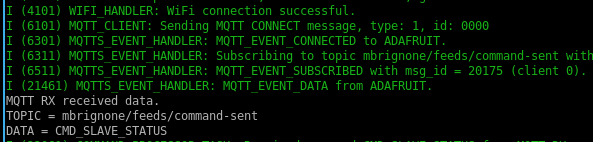
\includegraphics[width=\textwidth]{./Figures/output_mqtt_connection.png}
\caption{Eventos disparados en el microcontrolador por la comunicación utilizando MQTT.}
\label{fig:output_mqtt_connection}
\end{figure}

Primero se espera a que el \emph{driver} WiFi indique que la conexión ya está habilitada, y luego se envía la orden de conectarse al \emph{broker} MQTT, disparándose a continuación el evento MQTT\_EVENT\_CONNECTED, el cual indica que la conexión al \emph{broker} fue exitosa. 

Para detectar los comandos enviados por el usuario, el cliente se suscribe al \emph{topic} correspondiente, lo cual dispara el evento MQTT\_EVENT\_SUBSCRIBED.

Finalmente, se dispara el evento MQTT\_EVENT\_DATA indicando que hay un dato nuevo en el \emph{topic} al cual el microcontrolador se encuentra suscrito, y se puede ver que el dato recibido se corresponde al comando enviado desde Adafruit.

\subsubsection{Comunicación con el fabricante}

La comunicación con el fabricante consiste en el envío de datos desde el microcontrolador hacia Google Cloud utilizando el protocolo MQTT. Para ello primero el dispositivo debe conectarse al \emph{broker} de Google Cloud y autenticarse mediante un JSON Web Token, tal como se explicó en la sección \ref{sec:google_cloud}. Este proceso se puede observar en la figura \ref{fig:output_gcloud_connection}, donde se aprecia cómo se generó el JWT, para lo cual se obtuvo el tiempo actual mediante el protocolo SNTP, y luego se conectó a Google Cloud.

\begin{figure}[h]
\centering
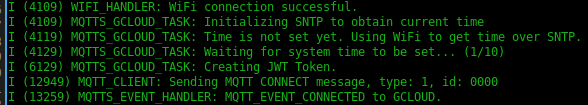
\includegraphics[width=\textwidth]{./Figures/output_gcloud_connection.png}
\caption{Conexión del microcontrolador a Google Cloud por MQTT.}
\label{fig:output_gcloud_connection}
\end{figure}

Una vez conectado al \emph{broker}, se enviaron algunos mensajes y luego se revisó el registro de eventos (\emph{logs}) de Google Cloud para verificar que la comunicación fue exitosa. Esto se ilustra en la figura \ref{fig:gcloud_log}, en la que se ve que primero se produce la conexión de un dispositivo, luego la publicación de dos mensajes y finalmente la desconexión del dispositivo. Cabe mencionar que en el registro se cuenta con mucha más información que la mostrada en la figura \ref{fig:gcloud_log}, pero se la omite por simplicidad.

\begin{figure}[h]
\centering
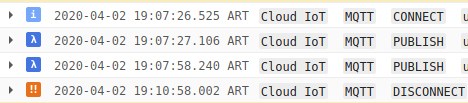
\includegraphics[width=\textwidth]{./Figures/gcloud_log.png}
\caption{Registro de eventos MQTT en Google Cloud.}
\label{fig:gcloud_log}
\end{figure}

\subsubsection{Servidor web}

\subsection{Comunicación BLE}

\subsection{Comunicación serie con electrodoméstico}

\section{Integración del sistema}

\subsection{Visualización de datos en Google Cloud Platform}
























